\documentclass[12pt,onecolumn,a4paper,fleqn]{article}
\usepackage[top=1in, bottom=1in, left=0.75in, right=0.75in]{geometry}
\usepackage{epsfig,graphicx,amsthm,amsmath}
\usepackage[table,xcdraw,svgnames]{xcolor}
\usepackage{setspace}
\usepackage{mathtools}
\usepackage{fancyhdr}
\usepackage{sidecap}
\usepackage{caption}
\usepackage{subcaption}
\usepackage{hyperref}
\usepackage{tikz}
\usepackage{pgfplots}
\usetikzlibrary{decorations.pathreplacing}
\usepackage{relsize}
\usepackage{color,xcolor}
\usepackage[framed,numbered]{matlab-prettifier}
\usepackage{float}
\usepackage{enumerate}
\usepackage{booktabs}
\usepackage{wrapfig}
\usepackage{datetime}
\graphicspath{ {figures/} }
\usepackage{array}
\usepackage{xepersian}

\hypersetup{
	colorlinks=true,
	urlcolor=blue!70!black,
	linkcolor=blue
}


\settextfont[Path=fonts/,BoldFont={ZarBd.ttf},BoldFeatures={Scale=0.9}]{BZar.ttf}

%\DeclarePairedDelimiter\ceil{\lceil}{\rceil}
%\DeclarePairedDelimiter\floor{\lfloor}{\rfloor}

%\definecolor{vgreen}{RGB}{104,180,104}
%\definecolor{vblue}{RGB}{49,49,255}
%\definecolor{vorange}{RGB}{255,143,102}


% title page template
\newcommand{\heading}[2]
{
	\begin{center}
		{\huge
			\textbf{
				به نام خدا\\
			}
		}
		
		\vspace*{1.5cm}
		
\includegraphics[scale=0.9]{source/sharif_logo.png}\\
		\vspace*{0.5cm}
		{\Large
			\textbf{
				دانشگاه صنعتی شریف\\
				\vspace*{0.25cm}
				دانشکده مهندسی کامپیوتر\\
			}
		}
		\vspace*{3cm}
		{\huge
			\textbf{
				آزمایشگاه معماری کامپیوتر\\
				\vspace*{0.75cm}
			}
		}
		
		{\Large
			\textbf{
				#1:\\
				#2\\
			}
		}
		
		\noindent\rule[1ex]{\linewidth}{1pt}\\
		\vspace*{0.5cm}
		\begin{table}[H]
			\centering
			\begin{tabular}{|c|c|}
				\hline
				\multicolumn{2}{|c|}{\textbf{اطلاعات تیم}}
				\\ \hline
				\textbf{نام اعضا} & \textbf{شماره دانشجویی}
				\\ \hline
				متین داغیانی & 98106456
				\\ \hline
				بردیا محمدی & 98171104
				\\ \hline
				محمدجواد هزاره & 98101074
				\\ \hline 
			\end{tabular}
		\end{table}
		{\Large				
			\vspace*{0.75cm}
			\textbf{
				پاییز 1400
		}}		
	\end{center}
}

\pagestyle{fancy}
\fancyhf{}
\rhead{\textbf{آزمایشگاه معماری کامپیوتر}}
%%--------------------[should change]---------------------
\chead{\textbf{گزارش آزمایش پنجم}}
%%--------------------[should change]---------------------
\lhead{\textbf{\nouppercase{\rightmark}}}
\cfoot{({\thepage})}
\renewcommand{\headrulewidth}{1pt}
\renewcommand{\footrulewidth}{1pt}
\renewcommand{\sectionmark}[1]{\markright{#1}}
\renewcommand{\subsectionmark}[1]{\markright{#1}}
%\newdateformat{monthyeardate}{%
	%	\monthname[\THEMONTH], \THEYEAR}

\onehalfspacing
\begin{document}
	%%% title pages
	\large
	\begin{titlepage}
		\heading{آزمایش پنجم}{طراحی واحد محاسبه}
		\thispagestyle{empty}
	\end{titlepage}	
	\pagebreak
	
	%%% contents page
	\tableofcontents
	\thispagestyle{empty}
	\pagebreak
	
	%%% figures page
	\listoffigures
	\thispagestyle{empty}
	\pagebreak
	
	%%% main document
	\section{هدف آزمایش}
	هدف این آزمایش پیاده‌سازی واحد محاسبه‌ی یک کامپیوتر بود. این واحد محاسبه که معماری آن در شکل \ref{fig:architec} آمده است، از توانایی جمع و تفریق هشت بیتی برخوردار است. عملیات‌هایی که این واحد می‌تواند انجام دهد به فرم
	$d = r \pm s$
	بوده که $d$ آدرس ثبات مقصد و $s$ آدرس ثبات مبدا خواهد بود. $r$ نیز آدرسی ثابت است که به یکی از ثبات‌ها اشاره می‌کند. (در این مدار این ثباتِ ثابتْ همان $R_0$ است.)
	\begin{figure}[H]
		\centering
		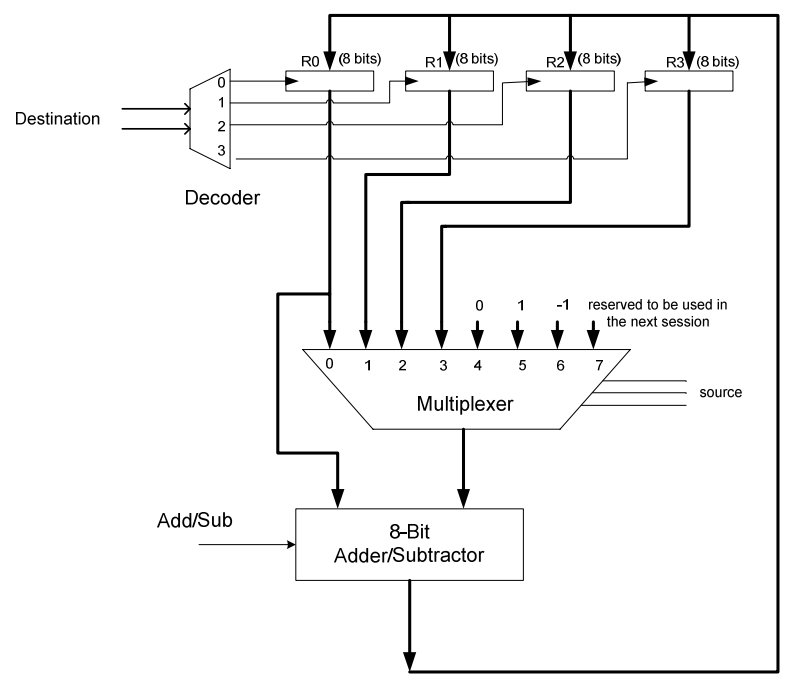
\includegraphics[width=0.68\textwidth]{source/architecture.png}
		\caption{معماری واحد محاسبه}
		\label{fig:architec}
	\end{figure}
	معماری دستورالعمل‌های این ماشین نیز در شکل \ref{fig:isa} آمده است.
	\begin{figure}[H]
		\centering
		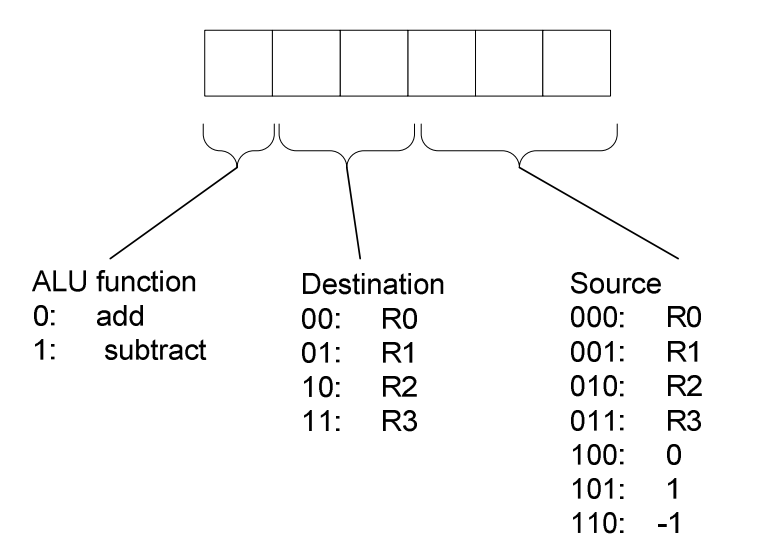
\includegraphics[width=0.45\textwidth]{source/isa.png}
		\caption{معماری مجموعه دستورالعمل‌ها}
		\label{fig:isa}
	\end{figure}
	همانطور که در تصویر دیده می‌شود بیت اول دستورالعمل مشخص کننده‌ی نوع عملیات بوده، دو بیت بعدی آدرس ثبات مقصد را مشخص می‌کنند و سه بیت آخر نیز آدرس ثبات مبدا هستند. نمای کلی مدار طراحی شده نیز در شکل \ref{fig:circuit} آمده است.
	\begin{figure}[H]
		\centering
		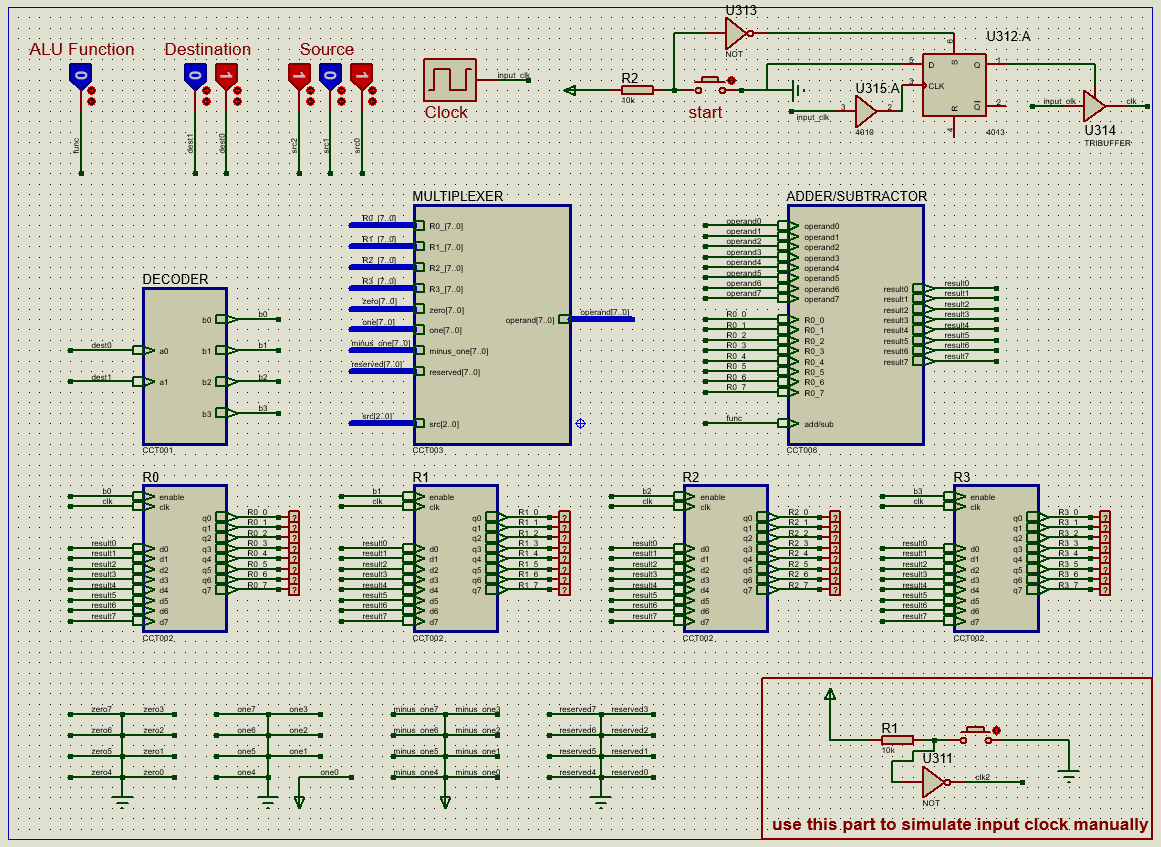
\includegraphics[width=0.85\textwidth]{source/circuit.png}
		\caption{نمای کلی مدار واحد محاسبه}
		\label{fig:circuit}
	\end{figure}
	در بخش بعدی به مراحل طراحی این مدار و بررسی طراحی داخلی ماژول‌های آن خواهیم پرداخت.
	\pagebreak
	\section{طراحی و پیاده‌سازی مدار}
	\subsection*{ماژول‌های مورد نیاز و شروع به کار مدار}
	همانطور که در شکل \ref{fig:architec} برای معماری مدار دیده می‌شود، به یک دیکودر برای تعیین آدرس ثبات مقصد، چهار ثبات هشت بیتی که قابلیت بارگذاری داشته باشند، یک مالتی پلکسر برای انتخاب ثبات مبدا و در نهایت ماژول جمع و تفریق کننده نیاز داریم. با فشردن کلید $start$ مدار آغاز به کار کرده و محسابه‌ی خود را انجام می‌دهد. با توجه به این که مدار ترکیبی است محاسبه‌ی آن یک کلاک به طول می‌انجام بنابراین کلاک داخلی آن را که باعث فعال شدن رجیسترها می‌شود با اندکی تاخیر پس از آمدن کلاک غیرفعال می‌کنیم. این فرآیند در قسمتی از مدار که در شکل زیر آمده است انجام شده است.
	\begin{figure}[H]
		\centering
		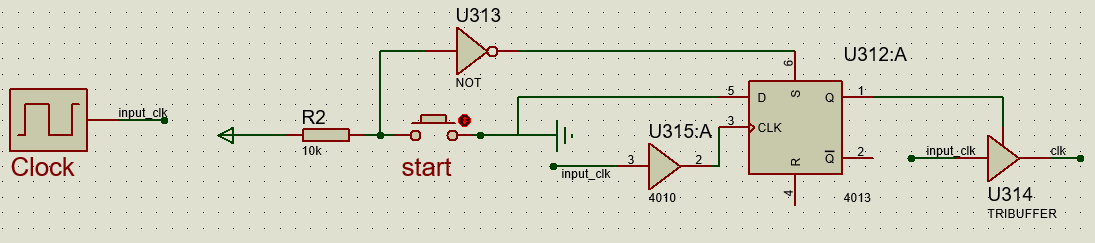
\includegraphics[width=0.85\textwidth]{source/start.png}
		\caption{کلید $start$ و شروع به کار مدار}
		\label{fig:start}
	\end{figure}
	\subsection{ماژول \lr{DECODER}}
	همانطور که قبل‌تر توضیح داده شد، این ماژول وظیفه‌ی تعیین ثبات مقصد را از روی آدرس آن بر عهده دارد. خروجی آن به عنوان سیگنال \lr{enable} به رجیسترها داده شده تا در صورت فعال بودن این سیگنال، رجیستر موردنظر فعال شده و عملیات نوشتن روی آن انجام شود. رابط ورودی و خروجی این ماژول را در شکل \ref{fig:decoder} می‌توان دید.
	\begin{figure}[H]
		\centering
		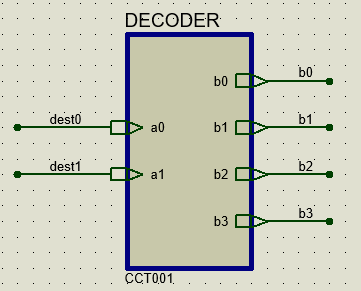
\includegraphics[width=0.45\textwidth]{source/decoder.png}
		\caption{ورودی و خروجی‌های \lr{DECODER}}
		\label{fig:decoder}
	\end{figure}
	همانطور که دیده می‌شود ورودی‌های آن بیت‌های دوم و سوم دستورالعمل هستند که با نام‌های $dest_0$ و $dest_1$ نام‌گذاری شده‌اند. طراحی داخلی این ماژول نیز به صورت شکل \ref{fig:decoder-in} است که به همان روش رایج ساخت دیکودر می‌باشد.
	\begin{figure}[H]
		\centering
		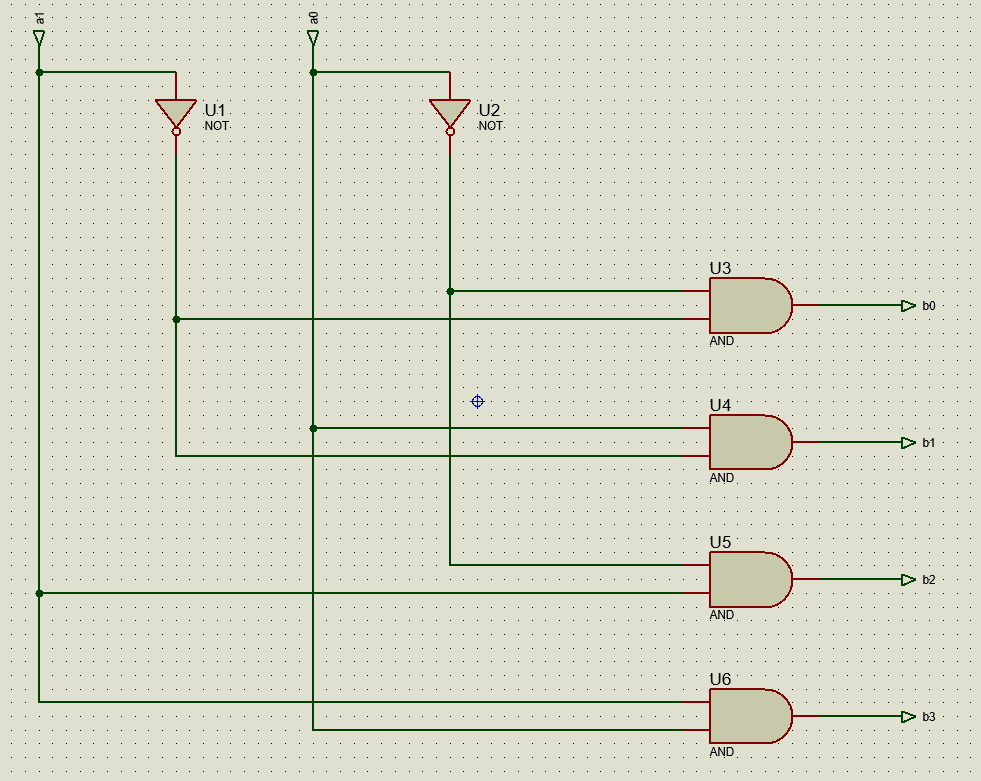
\includegraphics[width=0.7\textwidth]{source/decoder-in.png}
		\caption{طراحی داخلی ماژول \lr{DECODER}}
		\label{fig:decoder-in}
	\end{figure}
	\subsection{ثبات‌ها}
	این ماژول‌ها که در مدار با نام $R_0$ تا $R_3$ نام‌گذاری شده‌اند، ثبات‌های کامپیوتر را تشکیل می‌دهند. ورودی‌ها و خروجی‌های آن‌ها را در شکل \ref{fig:regs} می‌توان دید.
	\begin{figure}[H]
		\centering
		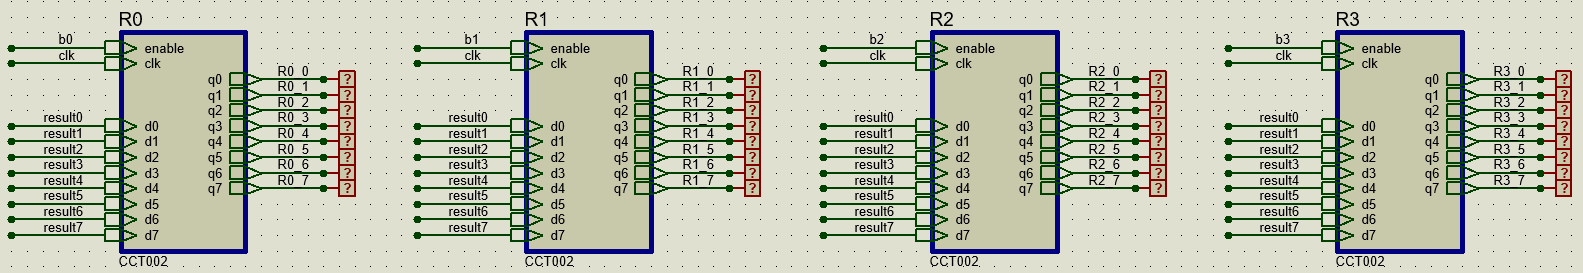
\includegraphics[width=0.95\textwidth]{source/regs.png}
		\caption{ورودی و خروجی‌های ثبات‌ها}
		\label{fig:regs}
	\end{figure}
	همانطور که در تصویر دیده می‌شود هر ماژول علاوه بر ورودی‌های $d_0$ تا $d_7$، ورودی $enable$ نیز دارد که با فعال شدن این سیگنال، ورودی‌های $d_0$ تا $d_7$ در رجیستر‌های این ماژول بارگذاری می‌شود. خروجی آن‌ها نیز همواره فعال و مقدار ذخیره شده در رجیستر‌های آن‌ها را نشان می‌دهد.
	
	برای طراحی داخلی هر یک از آن‌ها نیز از هشت فلیپ‌فلاپ نوع $D$ استفاده شده که طراحی آن را در شکل \ref{fig:regs-in} می‌توان مشاهده کرد.
	\begin{figure}[H]
		\centering
		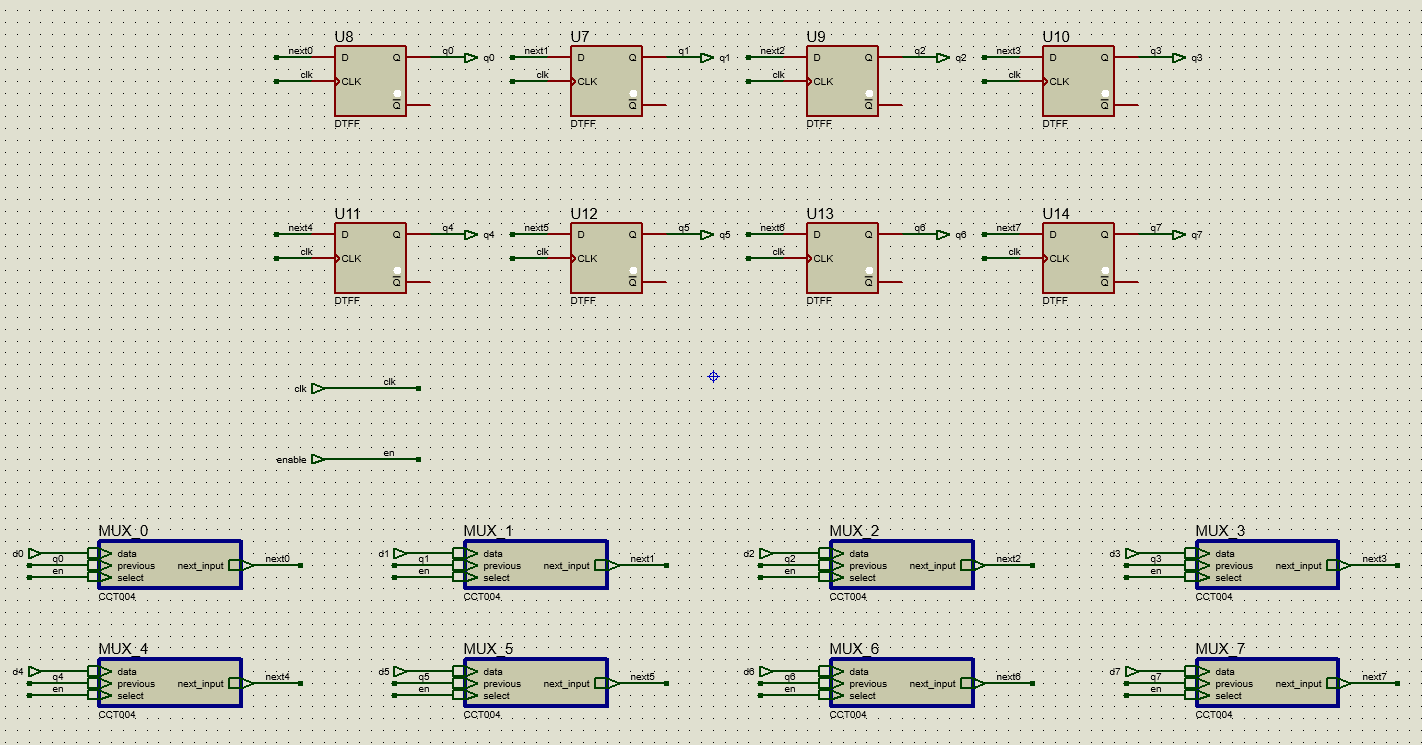
\includegraphics[width=0.7\textwidth]{source/regs-in.png}
		\caption{طراحی داخلی ثبات‌ها}
		\label{fig:regs-in}
	\end{figure}
	\noindent
	هم‌چنین از یک مالتی‌پلکسر برای مشخص کردن ورودی هر فلیپ‌فلاپ استفاده شده که تا زمانی که سیگنال $enable$ فعال نباشد، با هر کلاک رجیسترها همان مقدار قبلی خود را در خود نگه دارند. طراحی داخلی هر یک از این مالتی‌پلکسرهای 2به1 را در شکل \ref{fig:regs-mux} می‌توان دید.
	\begin{figure}[H]
		\centering
		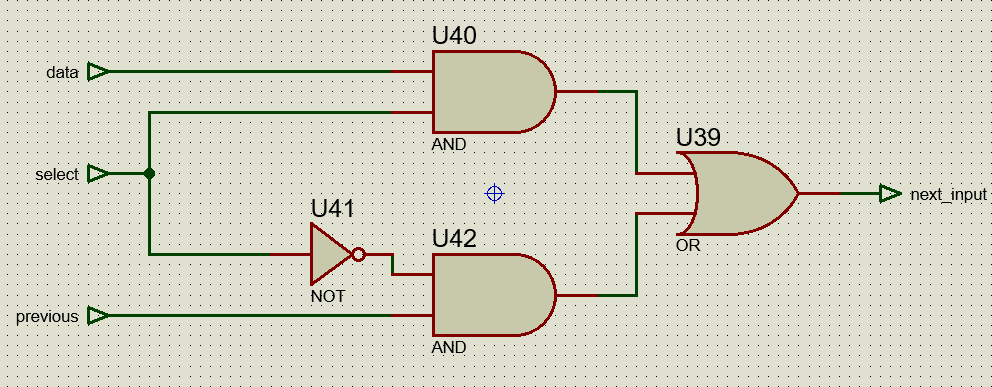
\includegraphics[width=0.6\textwidth]{source/regs-mux-in.png}
		\caption{طراحی داخلی مالتی‌پلکسر 2به1}
		\label{fig:regs-mux}
	\end{figure}
	\subsection{ماژول \lr{MULTIPLEXER}}
	از این ماژول برای تعیین یکی از عملوند‌های عملیت‌ها استفاده می‌شود. همانطور که قبلا اشاره شد، یکی از عملوند‌های این واحد محاسبه، ثابت بوده و از ثبات $R_0$ می‌آید و دیگری با استفاده از آدرسی که در دستورالعمل آمده است مشخص می‌شود. ورودی‌ها و خروجی‌های این ماژول را در شکل \ref{fig:multiplexer} می‌توان مشاهده کرد.
	\begin{figure}[H]
		\centering
		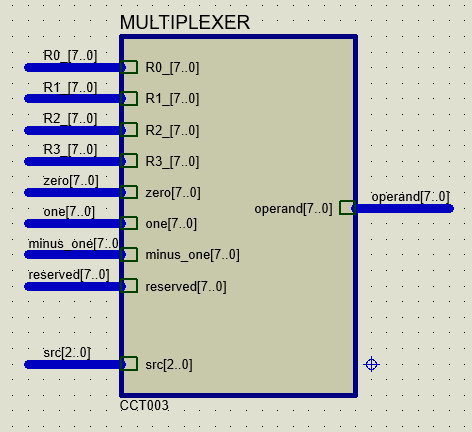
\includegraphics[width=0.5\textwidth]{source/multiplexer.png}
		\caption{ورودی و خروجی‌های \lr{MULTIPLEXER}}
		\label{fig:multiplexer}
	\end{figure}
	این ماژول یک مالتی‌پلکسر 8به1 است که در واقع هر ورودی آن خود هشت بیتی بوده و خروجی آن نیز هشت بیتی است. سیگنال انتخاب‌کننده‌ی آن نیز همانطور که در تصویر مشخص است از سه بیت آخر دستورالعمل می‌آید که با باس $src$ مشخص شده است. پیش از پرداختن به طراحی داخلی مدار باید توجه کنیم که این واحد توانایی جمع و تفریق با مقادیر ثابت $0$، $1$ و $-1$ را نیز داراست که به ترتیب اگر آدرس مبدا برابر $4$، $5$ و $6$ باشد این عملیات صورت می‌گیرد. برای همین منظور سه باس $zero$،
	$one$
	و
	$minus\_one$
	به ورودی‌های ۴ تا ۶ این ماژول داده شده‌اند. ساخت این باس‌ها نیز مطابق شکل \ref{fig:const-opr} صورت انجام شده است.
	\begin{figure}[H]
		\centering
		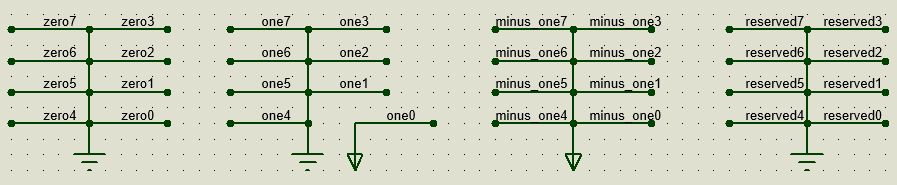
\includegraphics[width=0.85\textwidth]{source/const-operand.png}
		\caption{عملوند‌های ثابت}
		\label{fig:const-opr}
	\end{figure}
	در طراحی داخلی ماژول نیز با توجه به سیگنال‌ سلکتور، هر بیت ورودی‌های هشت بیتی به صورت جداگانه بررسی شده و انتخاب شده است. به عبارتی به ازای هر بیت سیگنال‌های ورودی، از یک مالتی‌پلکسر 8به1 استفاده شده که ورودی‌ها و خروجی آن یک بیتی است. طراحی داخلی این ماژل در شکل \ref{fig:mux8-in} آمده است.
	\begin{figure}[H]
		\centering
		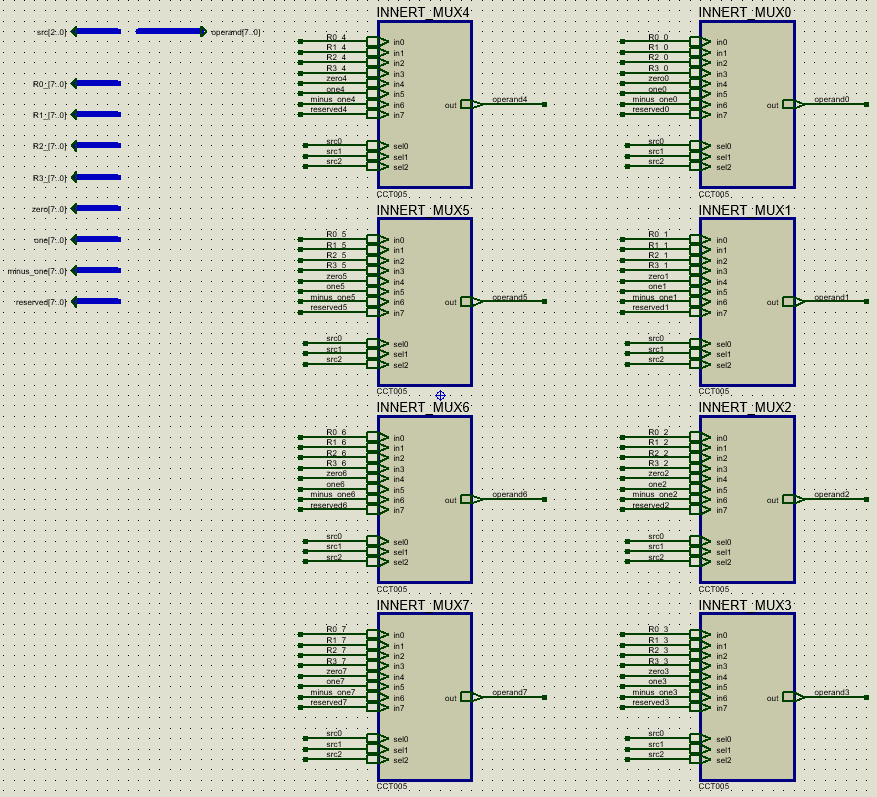
\includegraphics[width=0.65\textwidth]{source/multiplexer-in.png}
		\caption{طراحی داخلی ماژول \lr{MULTIPLEXER}}
		\label{fig:mux8-in}
	\end{figure}
	طراحی داخلی مالتی‌پلکسرهای ۸به۱ یک بیتی نیز در شکل \ref{fig:mux1bit-in} آمده است.
	\begin{figure}[H]
		\centering
		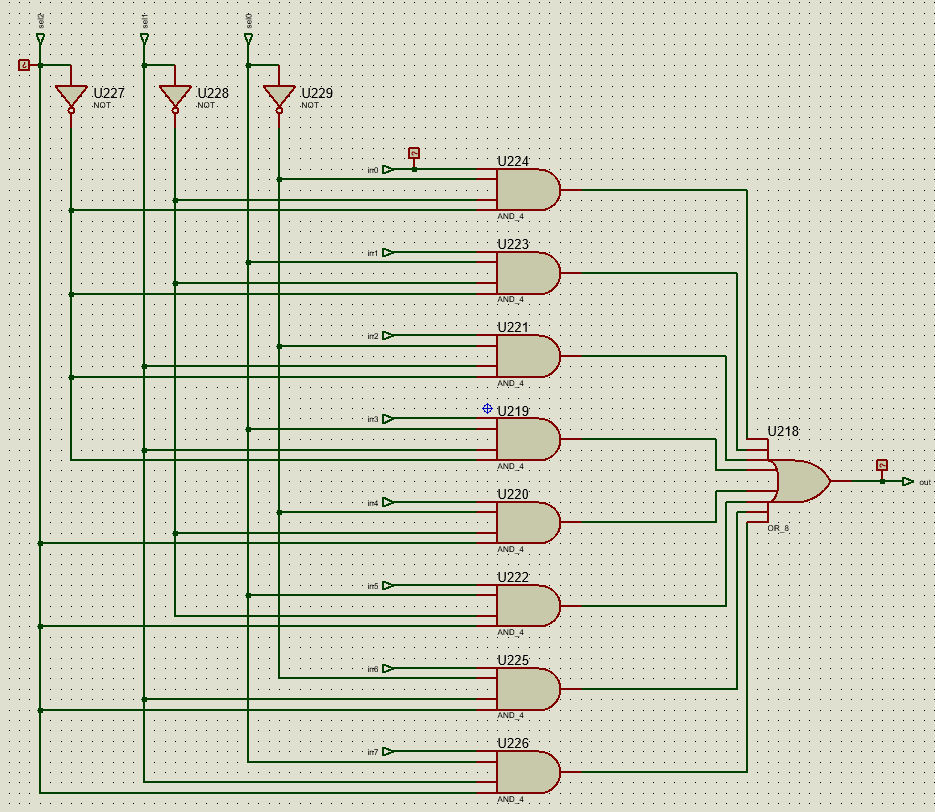
\includegraphics[width=0.65\textwidth]{source/inner-mux.png}
		\caption{طراحی داخلی ماژول‌های \lr{INNERT\_MUX} استفاده شده در شکل \ref{fig:mux8-in}}
		\label{fig:mux1bit-in}
	\end{figure}
	\subsection{ماژول \lr{ADDER/SUBTRACOTR}}
	این ماژول نیز وظیفه‌ی اصلی محاسبه را انجام می‌دهد. ورودی‌های آن هشت بیت رجیستر $R_0$ است که یکی از عملوند‌های عملیات را تشکیل داده و هشت ورودی دیگر از خروجی ماژول \lr{MULTIPLEXER} آمده‌اند که عملوند دوم عملیات را تشکیل می‌دهند. ورودی‌ها و خروجی‌های این مدار در شکل \ref{fig:adder} نشان داده شده است.
	\begin{figure}[H]
		\centering
		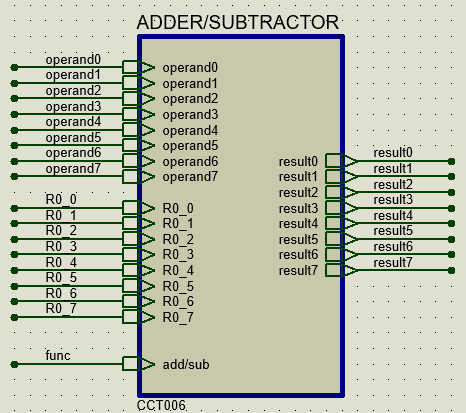
\includegraphics[width=0.4\textwidth]{source/adder.png}
		\caption{ورودی و خروجی‌های \lr{ADDER/SUBTRACTOR}}
		\label{fig:adder}
	\end{figure}
	سیگنال $add/sub$ نیز به بیت اول دستورالعمل متصل شده که مشخص می‌کند عملیات جمع یا تفریق است. برای طراحی داخلی این ماژول نیز از جمع‌کننده‌ی کامل (\lr{Full Adder}) استفاده شده که در شکل \ref{fig:adder-in} نیز طراحی داخلی آن نشان داده شده است.
	\begin{figure}[H]
		\centering
		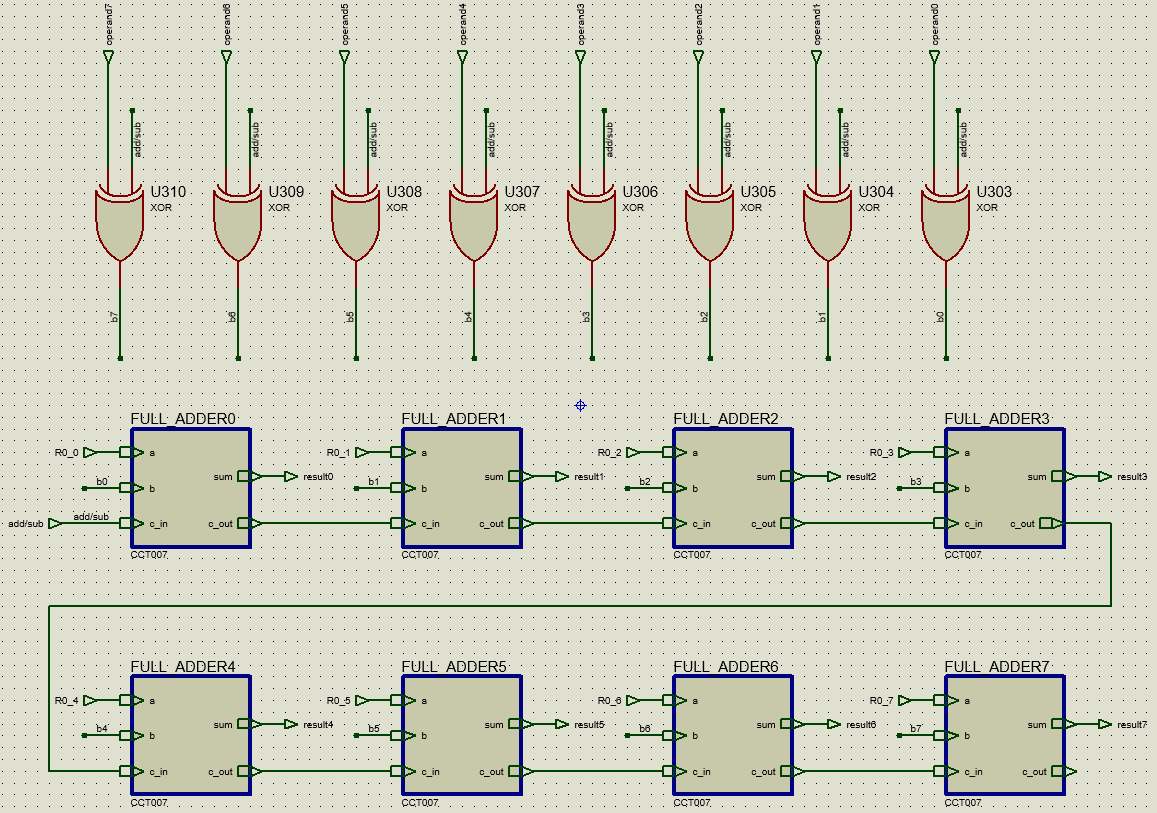
\includegraphics[width=0.7\textwidth]{source/adder-in.png}
		\caption{طراحی داخلی ماژول \lr{ADDER/SUBTRACTOR}}
		\label{fig:adder-in}
	\end{figure}
	برای تفریق از روش جمع با متمم دو استفاده شده که برای متمم دو کردن عملوندنیز بیت‌های آن در صورت یک بودن سیگنال $add/sub$ نات می‌شوند که این کار با $XOR$ کردن این بیت‌ها با سیگنال $add/sub$ صورت می‌گیرد و با اضافه شدن همین سیگنال به $c_in$ فول ادر اول، عدد مورد نظر متمم دو می‌شود. در ادامه جمع به صورت سری با استفاده از فول ادر ها انجام می‌شود. طراحی داخلی فول ادرها نیز در شکل \ref{fig:full-adder} نمایش داده شده است.
	\begin{figure}[H]
		\centering
		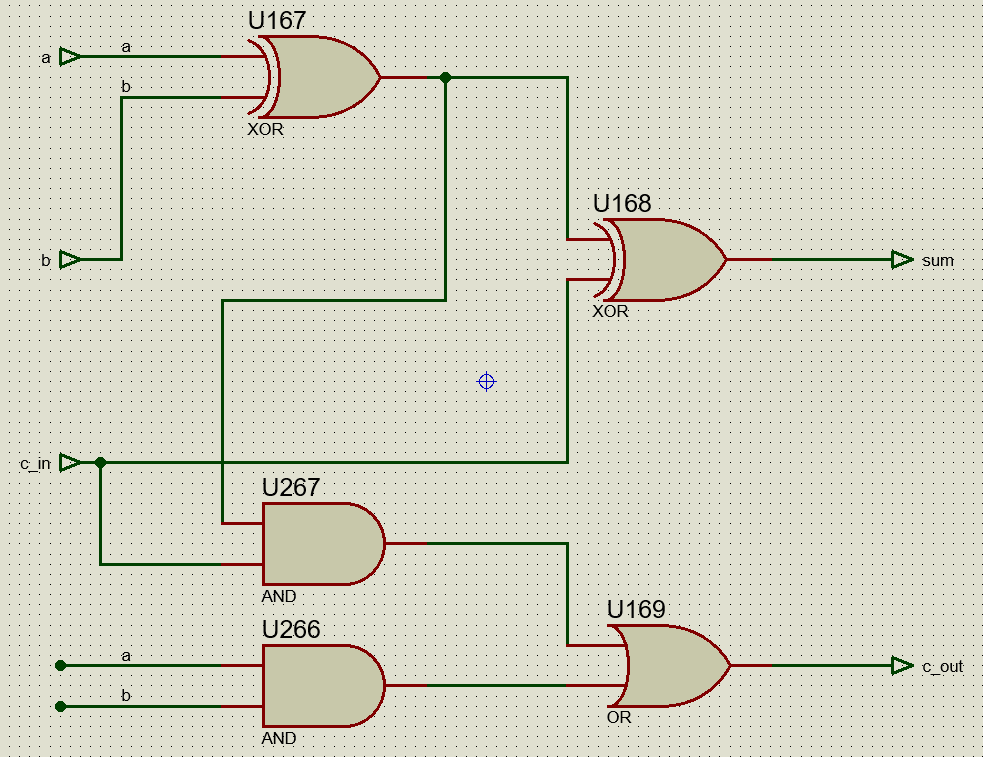
\includegraphics[width=0.45\textwidth]{source/full-adder.png}
		\caption{‌طراحی داخلی ماژول‌های \lr{FULL\_ADDER}}
		\label{fig:full-adder}
	\end{figure}
	\vspace*{7cm}
	\noindent
	در ادامه به تست مدار روی دستورالعمل‌های مختلف می‌پردازیم.
	\pagebreak
	\section{تست مدار}
	برای تست مدار، مجموعه دستورالعمل‌های زیر به صورت متوالی به مدار داده شده و شکل‌هایی که در ادامه می‌آیند وضعیت مدار را بعد از پردازش هر دستورالعمل نشان می‌دهند. هم‌چنین مقداری که هر ثبات بعد از اجرای هر دستورالعمل خواهد داشت در ادامه آمده است تا با مقداری که از مدار خروجی می‌گیریم مقایسه شود.
	\[
	\begin{aligned}
		001101 &\qquad (ADD,\;R1\;,1)	&&\to \{R0=0,&&R1=1,&&R2=0,&&R3=0\}\\
		010110 &\qquad (ADD,\;R2\;,-1)	&&\to \{R0=0,&&R1=1,&&R2=-1,&&R3=0\}\\
		100001 &\qquad (SUB,\;R0,\;R1)	&&\to \{R0=-1,&&R1=1,&&R2=-1,&&R3=0\}\\
		011010 &\qquad (ADD,\;R3,\;R2)	&&\to \{R0=-1,&&R1=1,&&R2=-1,&&R3=-2\}\\
		001000 &\qquad (ADD,\;R1,\;0)	&&\to \{R0=-1,&&R1=0,&&R2=-1,&&R3=-2\}\\
		100110 &\qquad (SUB,\;R0,-1)	&&\to \{R0=0,&&R1=0,&&R2=-1,&&R3=-2\}\\
		110011 &\qquad (SUB,\;R2,\;R3)	&&\to \{R0=0,&&R1=0,&&R2=2,&&R3=-2\}
	\end{aligned}
	\]
	و خروجی‌های مدار به صورت زیر خواهد بود:
	\begin{figure}[H]
		\centering
		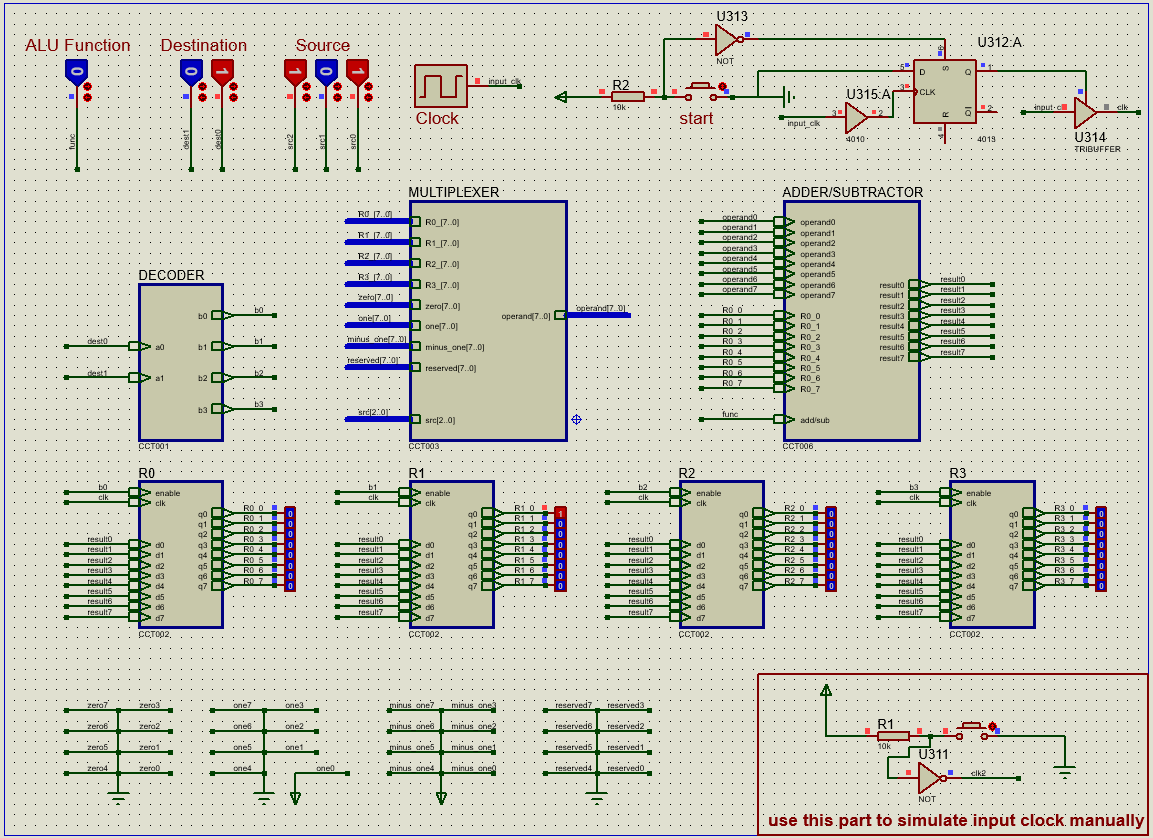
\includegraphics[width=0.8\textwidth]{source/inst1.png}
		\caption{‌وضعیت مدار پس از پردازش
			$001101$}
	\end{figure}
	\begin{figure}[H]
		\centering
		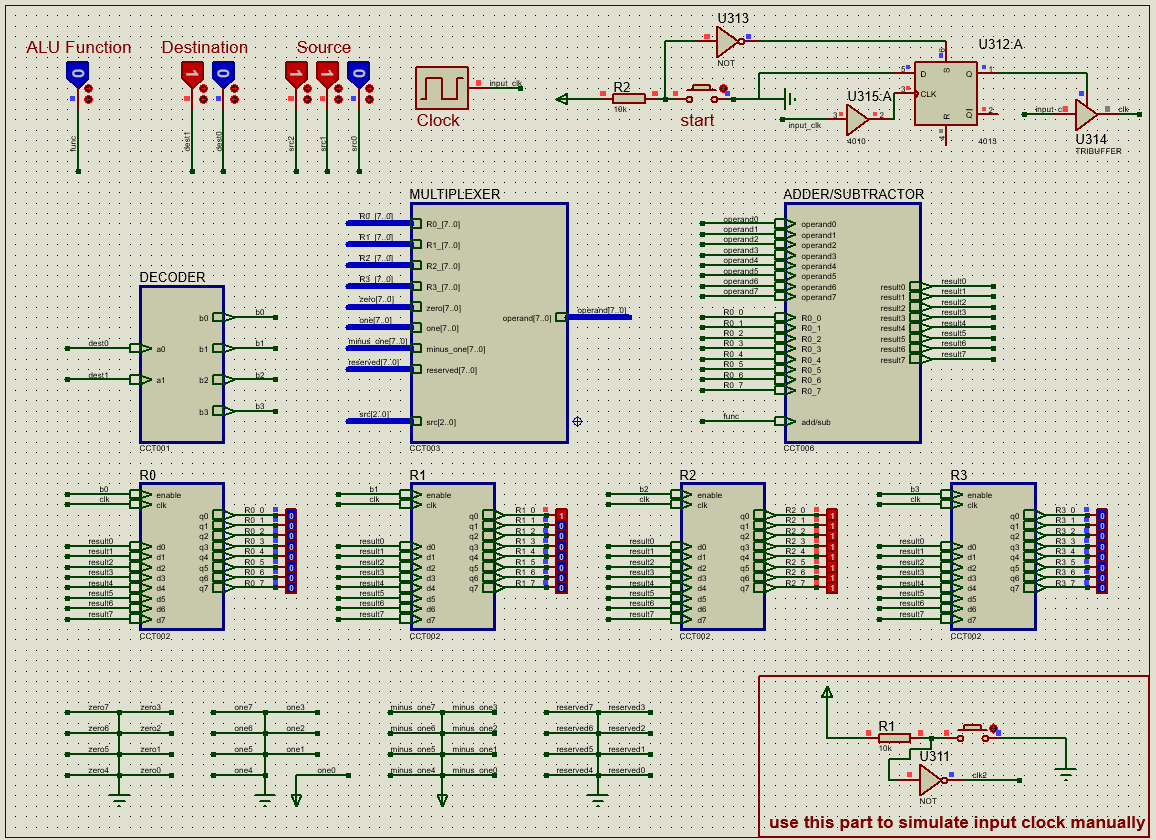
\includegraphics[width=0.8\textwidth]{source/inst2.png}
		\caption{‌وضعیت مدار پس از پردازش
			$010110$}
	\end{figure}
	\begin{figure}[H]
		\centering
		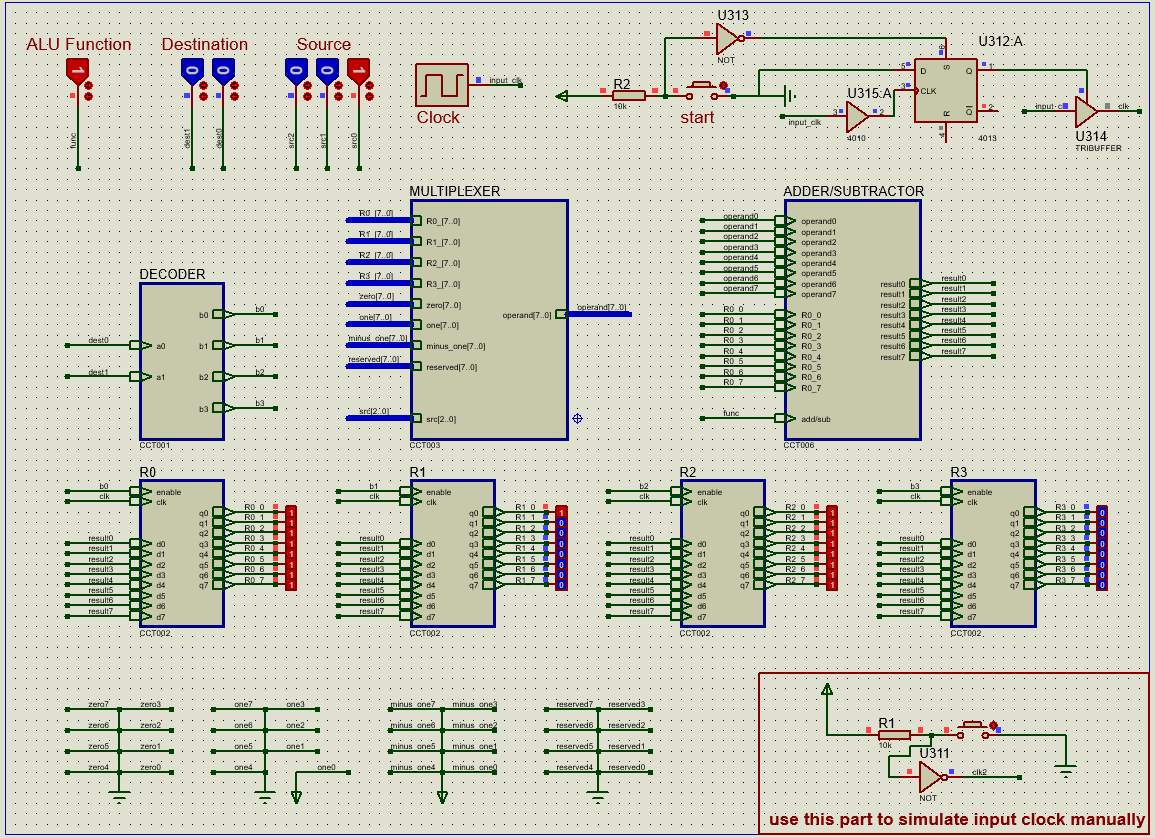
\includegraphics[width=0.8\textwidth]{source/inst3.png}
		\caption{‌وضعیت مدار پس از پردازش
			$100001$}
	\end{figure}
	\begin{figure}[H]
		\centering
		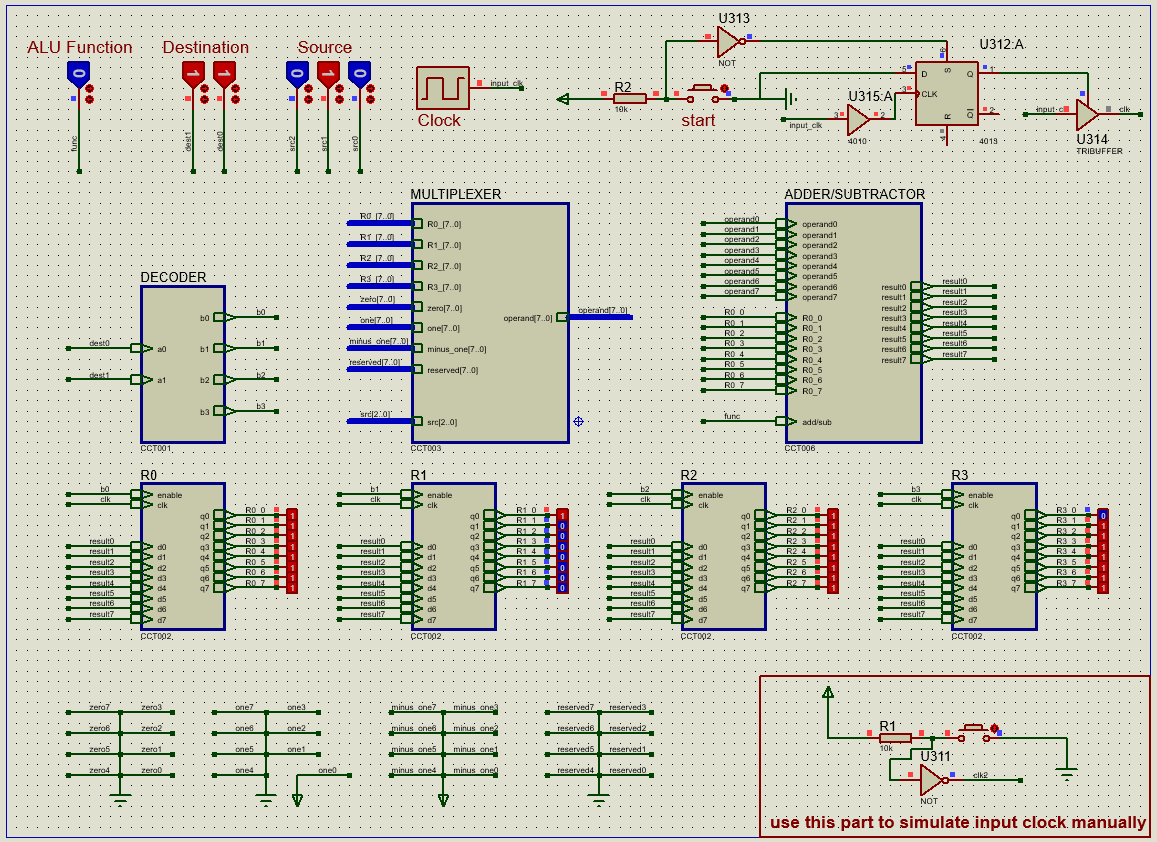
\includegraphics[width=0.8\textwidth]{source/inst4.png}
		\caption{‌وضعیت مدار پس از پردازش
			$011010$}
	\end{figure}
	\begin{figure}[H]
		\centering
		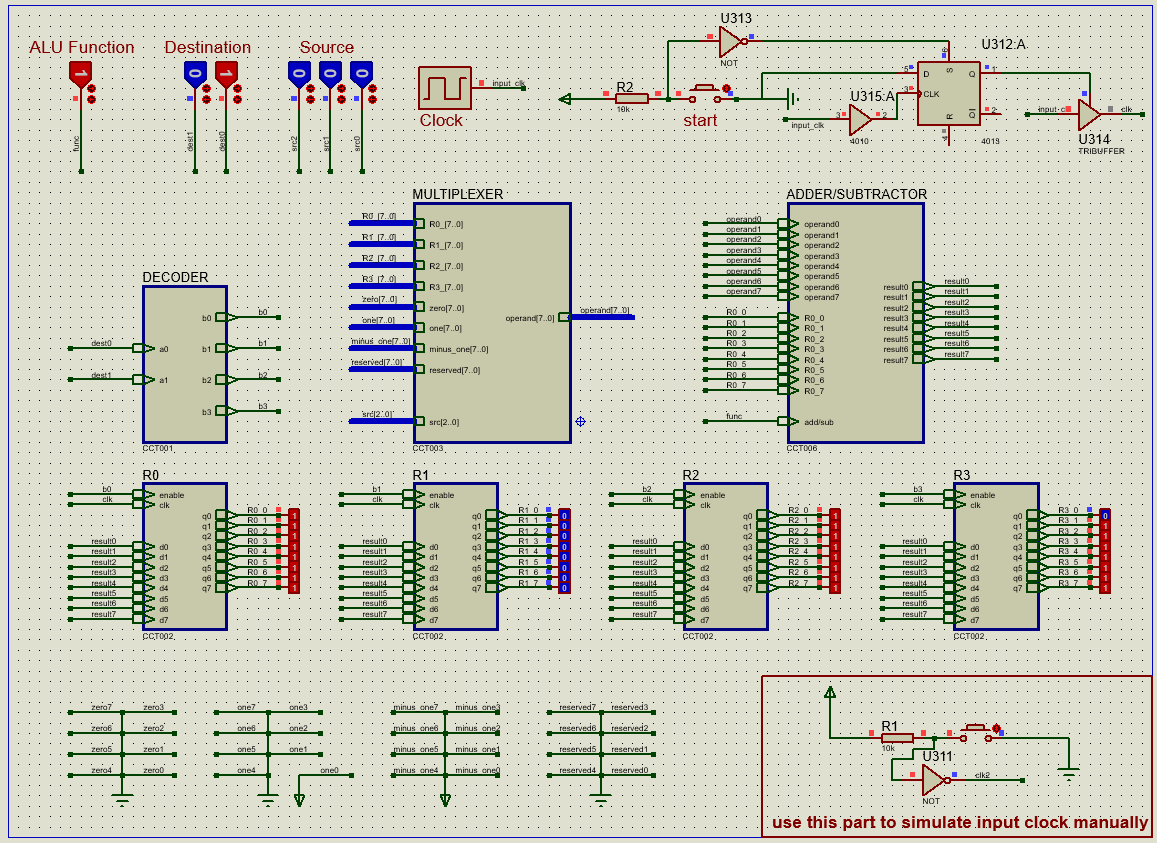
\includegraphics[width=0.8\textwidth]{source/inst5.png}
		\caption{‌وضعیت مدار پس از پردازش
			$001000$}
	\end{figure}
	\begin{figure}[H]
		\centering
		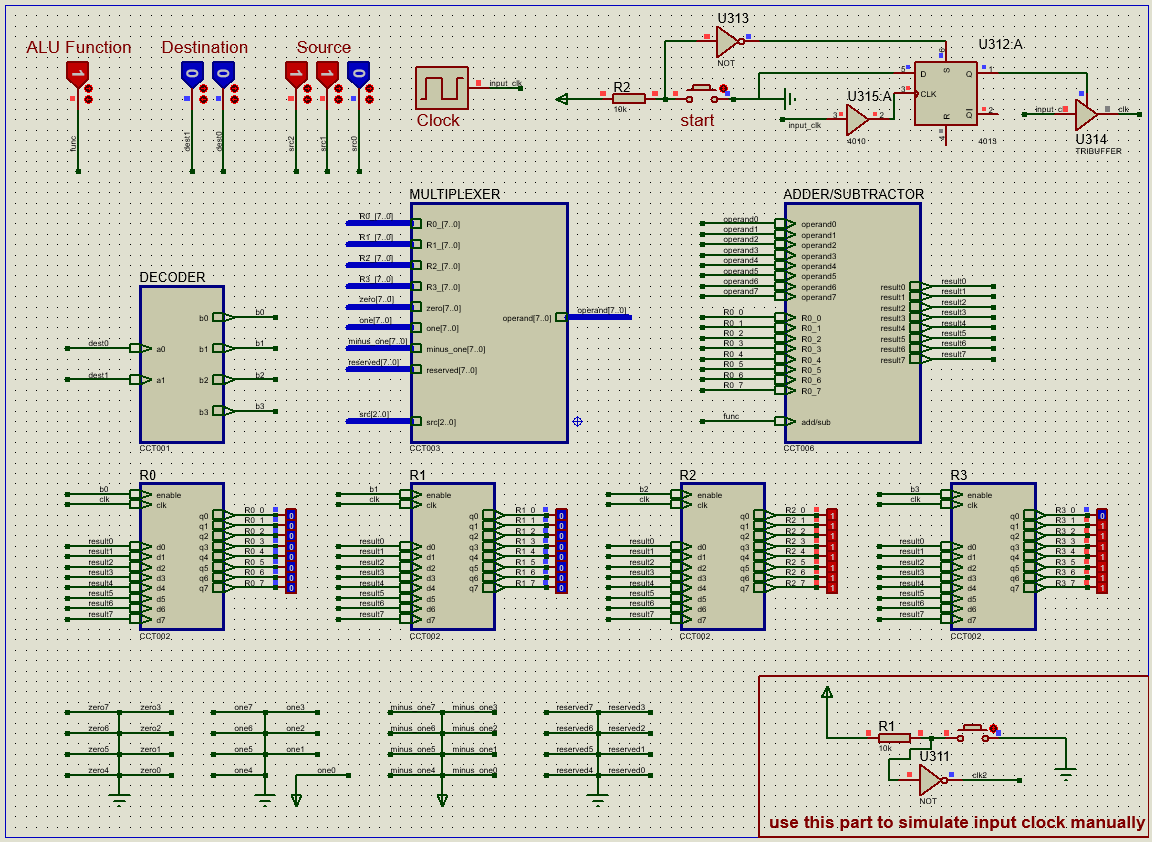
\includegraphics[width=0.8\textwidth]{source/inst6.png}
		\caption{‌وضعیت مدار پس از پردازش
			$100110$}
	\end{figure}
	\begin{figure}[H]
		\centering
		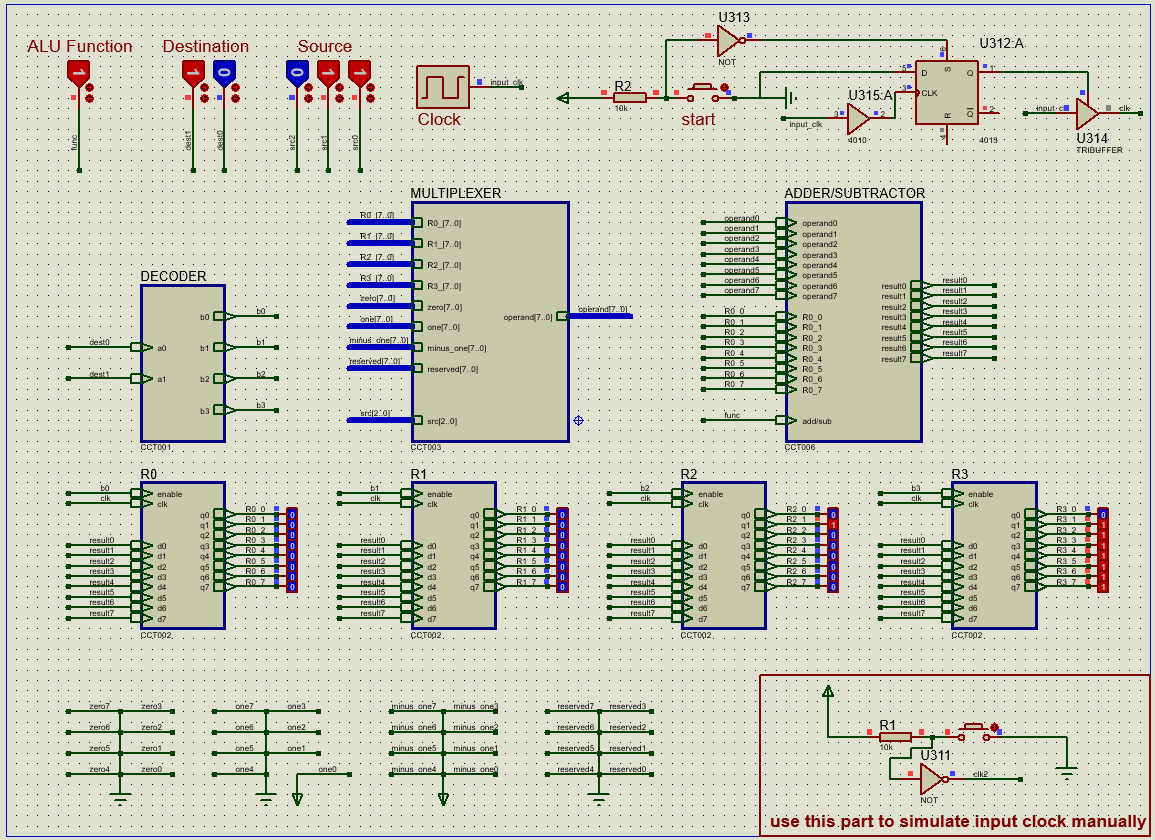
\includegraphics[width=0.8\textwidth]{source/inst7.png}
		\caption{‌وضعیت مدار پس از پردازش
			$110011$}
	\end{figure}	
\end{document}


